\section{Results}
\label{sec:results}
\paragraph{Performance metrics}
\Cref{tab:scores-dialog} and \Cref{tab:scores-narration} show
the performance of several model configurations on the retrieval and
triplet tasks on the dialog and narration datasets respectively.

In the case of the narration data this scores is not confounded by
speaker-based clues, which is an indication that the model possibly
learned to detect some aspects of utterance meaning. We investigate
this hypothesis further using multiple representational similarity
analysis.
 

 \begin{table}
   \centering
   \begin{tabular}{rlrr}
\toprule
 ID & Pretraining &  Recall@10 &  Triplet Acc \\
\midrule
 43 &          AV &      0.193 &        0.814 \\
 44 &           V &      0.084 &        0.728 \\
 45 &        None &      0.034 &        0.597 \\
\bottomrule
\end{tabular}

   \caption{Retrieval and triplet scores on dialog validation data.}
   \label{tab:scores-dialog}
 \end{table}

\begin{table}
   \centering
   \begin{tabular}{rlrr}
\toprule
 ID & Pretraining &  Recall@10 &  Triplet Acc \\
\midrule
 43 &          AV &      0.239 &        0.866 \\
 44 &           V &      0.166 &        0.822 \\
 45 &        None &      0.087 &        0.741 \\
\bottomrule
\end{tabular}

   \caption{Retrieval and triplet scores on narration validation data.}
   \label{tab:scores-narration}
 \end{table}
 
 
\paragraph{Multiple representational similarity analysis}

\Cref{tab:dialogvarcor} and \Cref{tab:narrationvarcor} show the raw
correlations between variables in the multiple RSA analysis, while
\Cref{fig:coef_dialog} and \Cref{fig:coef_narration} show the
standardized regression coefficients, where the target variable is
pairwise representation similarity for the pre-trained-only and the
fully-trained versions of the target model.

\begin{figure}
  \centering
  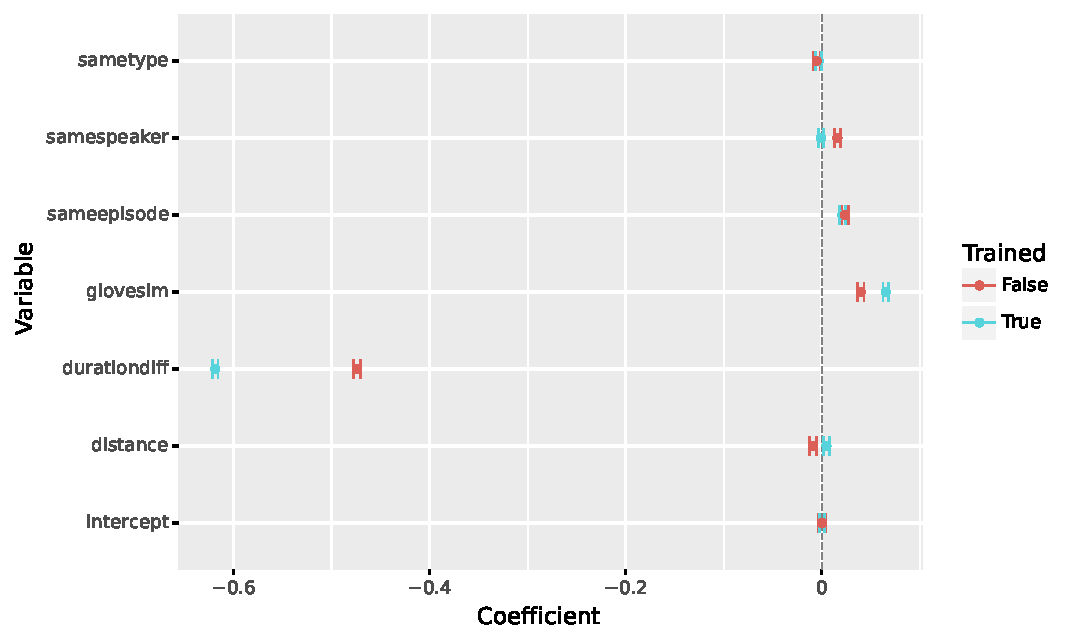
\includegraphics[scale=0.66]{results/grsa_dialog_coef.pdf}
  \caption{Association of predictors with trained and untrained
    model-based pairwise similarity scores for single-word utterances
    in the dialog validation data. Coefficients are standardized.}
  \label{fig:coef_dialog}
\end{figure}

\begin{figure}
  \centering
  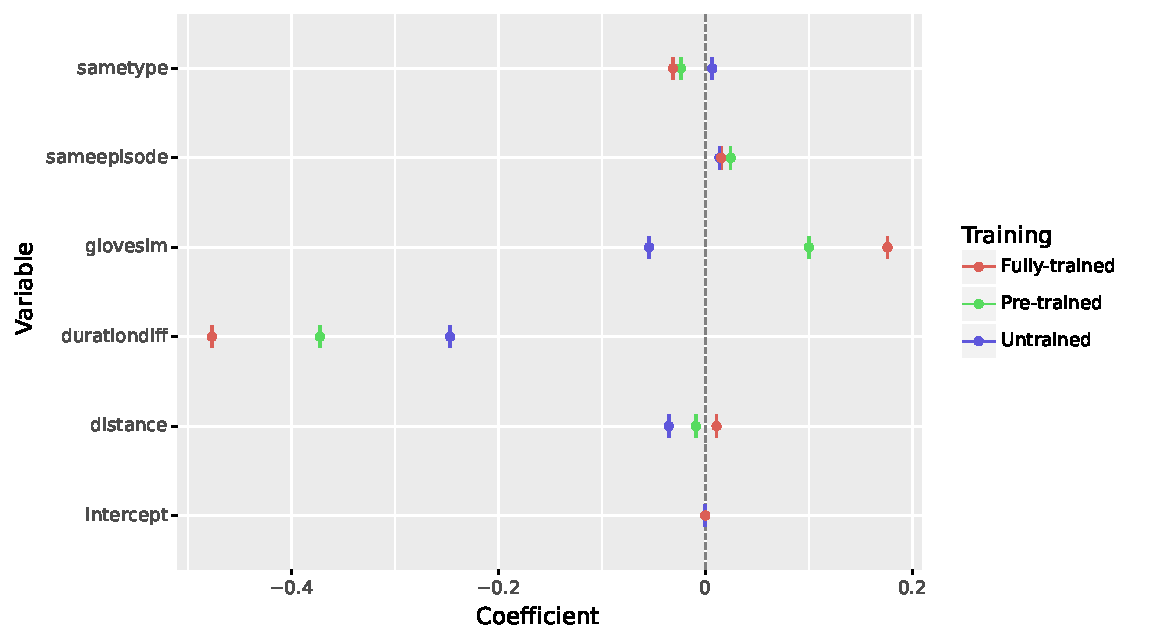
\includegraphics[scale=0.66]{results/grsa_narration_coef.pdf}
  \caption{Association of predictors with trained and untrained
    model-based pairwise similarity scores for single-word utterances
    in the narration validation data. Coefficients are standardized.}
  \label{fig:coef_narration}
\end{figure}


For both data subsets (dialog and narration), the highest magnitude
predictors are {\tt durationdiff} and {\tt glovesim}. The effect of
the {\tt samespeaker} predictor for the dialog data is close to zero.
These effect are there already for the pre-trained-only
representations, but are strengthened for the fully-trained target
model.  This results indicate that the model learns some aspects of
word-level semantics as captured by GloVe word vectors, and that
speaker identity does not appear to be a substantial impact on
utterance embeddings.

Perhaps unexpectedly, the predictor meant to capture phonemic distance
{\tt distance} is not strongly associated with utterance similarity,
although it should be noted that here we are only investigating model
embeddings after the final attention pooling layer.

The strength of the association between differences in utterance
duration {\tt durationdiff} and pairwise similarities apparent in this
data was suprising and possibly undesirable. We conjecture that is
arises as an effect of the positional encodings in the transformer
layers.

